% ==========================================================
% Póster académico A1 horizontal · 3 columnas (referencias al final de la última)
% Maestría en Inteligencia Artificial Aplicada
%
% - Texto de contenido: fuente por defecto de LaTeX (Latin Modern).
% - Títulos y encabezados: serif de display.
% - Encabezados de sección: verde #9AA542.
%
% Compilación:
%   - pdfLaTeX (por defecto): Charter para títulos.
%   - XeLaTeX / LuaLaTeX: "Instrument Serif" para títulos si está
%     instalada (o subida a Overleaf); si no, TeX Gyre Pagella.
% ==========================================================
\documentclass[10pt]{article}

\usepackage{iftex}
\usepackage[a1paper,landscape,margin=1.5cm]{geometry}
\usepackage[spanish,es-noshorthands]{babel}
\usepackage{xcolor}
\usepackage{graphicx}
\usepackage{tikz}
\usetikzlibrary{arrows.meta}
\usepackage[most]{tcolorbox}
\usepackage{lipsum}
\usepackage{mwe}            % imágenes de ejemplo (example-image-a, ...)
\usepackage{enumitem}
\usepackage{booktabs}
\usepackage{colortbl}
\usepackage{microtype}

% ---------------------- TIPOGRAFÍA -------------------------
% Texto: fuente por defecto (Latin Modern). Títulos: \serif.
\ifTUTeX
  \usepackage{fontspec}
  \IfFontExistsTF{Instrument Serif}%
    {\newfontfamily\serif{Instrument Serif}}%
    {\newfontfamily\serif{TeX Gyre Pagella}}
\else
  \usepackage[utf8]{inputenc}
  \usepackage[T1]{fontenc}
  \usepackage{lmodern}      % fuentes escalables (evita avisos de tamaños)
  \usepackage[scaled=0.95]{helvet}
  \newcommand{\serif}{\fontfamily{bch}\selectfont}
\fi

\pagestyle{empty}
\setlength{\parindent}{0pt}
\setlength{\parskip}{0.4em}

% ---------------------- PALETA -----------------------------
\definecolor{olive}{HTML}{9AA542}        % encabezados de sección
\definecolor{olivedark}{HTML}{1B2208}    % títulos / texto de encabezados
\definecolor{olivelink}{HTML}{6B7A1F}    % acentos
\definecolor{olivesoft}{HTML}{E4E8C7}    % círculos / fondos suaves
\definecolor{ink}{HTML}{1A1A10}          % texto
\definecolor{muted}{HTML}{6B6B5E}
\definecolor{pagebg}{HTML}{FFFFFF}       % usa F8F8F3 para fondo crema

\pagecolor{pagebg}
\color{ink}

% ---------------------- DATOS DEL PÓSTER -------------------
\newcommand{\programa}{Maestría en Inteligencia Artificial Aplicada}
\newcommand{\tituloA}{Título del proyecto en dos líneas}
\newcommand{\tituloB}{aplicando inteligencia artificial}
\newcommand{\autores}{Nombre Apellido\quad Nombre Apellido\quad Nombre Apellido}
\newcommand{\asesor}{Dr./Dra. Nombre del Asesor}
\newcommand{\fecha}{Noviembre 2026}

% Logos (archivos: logo_izq.png / logo_der.png)
% Si no se permite la incorporación del logo de la empresa, usar el de MNA incluido en la carpeta
\newcommand{\logoizq}{%
  \IfFileExists{logo.jpeg}%
  {
\includegraphics[height=5cm]{logo.jpeg}}%
  {\tikz\node[draw=olive,dashed,line width=1.2pt,minimum width=10cm,
    minimum height=6cm,align=center,text=muted]{\Huge LOGO\\IZQUIERDO};}}
\newcommand{\logoder}{%
  \IfFileExists{logo_der.png}%
  {\includegraphics[height=5cm]{logo_der.png}}%
  {\tikz\node[draw=olive,dashed,line width=1.2pt,minimum width=10cm,
    minimum height=6cm,align=center,text=muted]{\Huge LOGO EMPRESA\\(si no se permite, incluir el de MNA)};}}

% ---------------------- ESTILOS ----------------------------
% Barra de sección (serif, texto oscuro sobre verde)
\newcommand{\seccion}[1]{%
  \begin{tcolorbox}[colback=olive,colframe=olive,arc=0pt,
    boxrule=0pt,left=8pt,top=3pt,bottom=4pt,width=\linewidth]
    {\serif\color{white}\fontsize{30}{36}\selectfont #1}
  \end{tcolorbox}\vspace{-0.3em}}

% Texto base (fuente por defecto de LaTeX)
\newcommand{\cuerpo}{\fontsize{24}{31}\selectfont}

% Círculo de contribución
\newcommand{\circulo}[1]{%
  \tikz\node[circle,fill=olivesoft,minimum size=6cm,align=center,
    text width=5cm,text=olivedark,
    font=\sffamily\bfseries\fontsize{19}{23}\selectfont]{#1};}

% Alturas del diseño (ajusta si cambias el tamaño del encabezado)
\newlength{\hdrh}\setlength{\hdrh}{9cm}      % encabezado
\newlength{\colh}
\setlength{\colh}{\dimexpr\textheight-\hdrh-6cm\relax}

% ======================================================
\begin{document}

% ---------------------- ENCABEZADO ------------------------
\noindent\parbox[t][\hdrh][c]{\linewidth}{%
\begin{minipage}[c]{0.20\linewidth}
  \raggedright\logoizq
\end{minipage}%
\begin{minipage}[c]{0.60\linewidth}
  \centering
  {\serif\fontsize{58}{65}\selectfont\color{olivedark}%
   \tituloA\\\tituloB\par}
  \vspace{0.5em}
  {\sffamily\bfseries\fontsize{30}{36}\selectfont\color{olivelink}\programa\par}
  \vspace{0.3em}
  {\fontsize{26}{32}\selectfont\color{ink}\autores\par}
  {\fontsize{22}{28}\selectfont\color{muted}Asesor: \asesor\ \textperiodcentered\ \fecha\par}
\end{minipage}%
\begin{minipage}[c]{0.20\linewidth}
  \raggedleft\logoder
\end{minipage}}

\vspace{0.4cm}
{\color{olive}\rule{\linewidth}{2.5pt}}
\vspace{0.6cm}

% ---------------------- COLUMNAS --------------------------
\noindent
\begin{minipage}[t][\colh][s]{0.30\linewidth}\cuerpo\vspace{0pt}
% ===== COLUMNA IZQUIERDA =====

\seccion{Contexto de negocio y problema}
\lipsum[1][1-8]

\lipsum[2][1-6]

\lipsum[3][1-4]

\begin{center}
  \begin{tikzpicture}
    \fill[olivesoft] (0,0) arc (180:0:4.5 and 4.5) -- (6,0) arc (0:180:3 and 3) -- cycle;
    \node[font=\serif\fontsize{64}{68}\selectfont,text=olivedark] at (4.5,1.1) {43\%};
  \end{tikzpicture}
\end{center}

\vfill
\seccion{Datos y preparación}
\begin{itemize}[leftmargin=1.2em,itemsep=0.5em]
  \item \lipsum[3][1-3]
  \item \lipsum[4][1-3]
  \item \lipsum[5][1-3]
\end{itemize}

\vfill
\seccion{Metodología y modelos}
\begin{itemize}[leftmargin=1.2em,itemsep=0.5em]
  \item \lipsum[6][1-3]
  \item \lipsum[7][1-3]
  \item \lipsum[12][1-3]
\end{itemize}

\end{minipage}\hfill
\begin{minipage}[t][\colh][s]{0.37\linewidth}\cuerpo\vspace{0pt}
% ===== COLUMNA CENTRAL =====

\begin{center}
  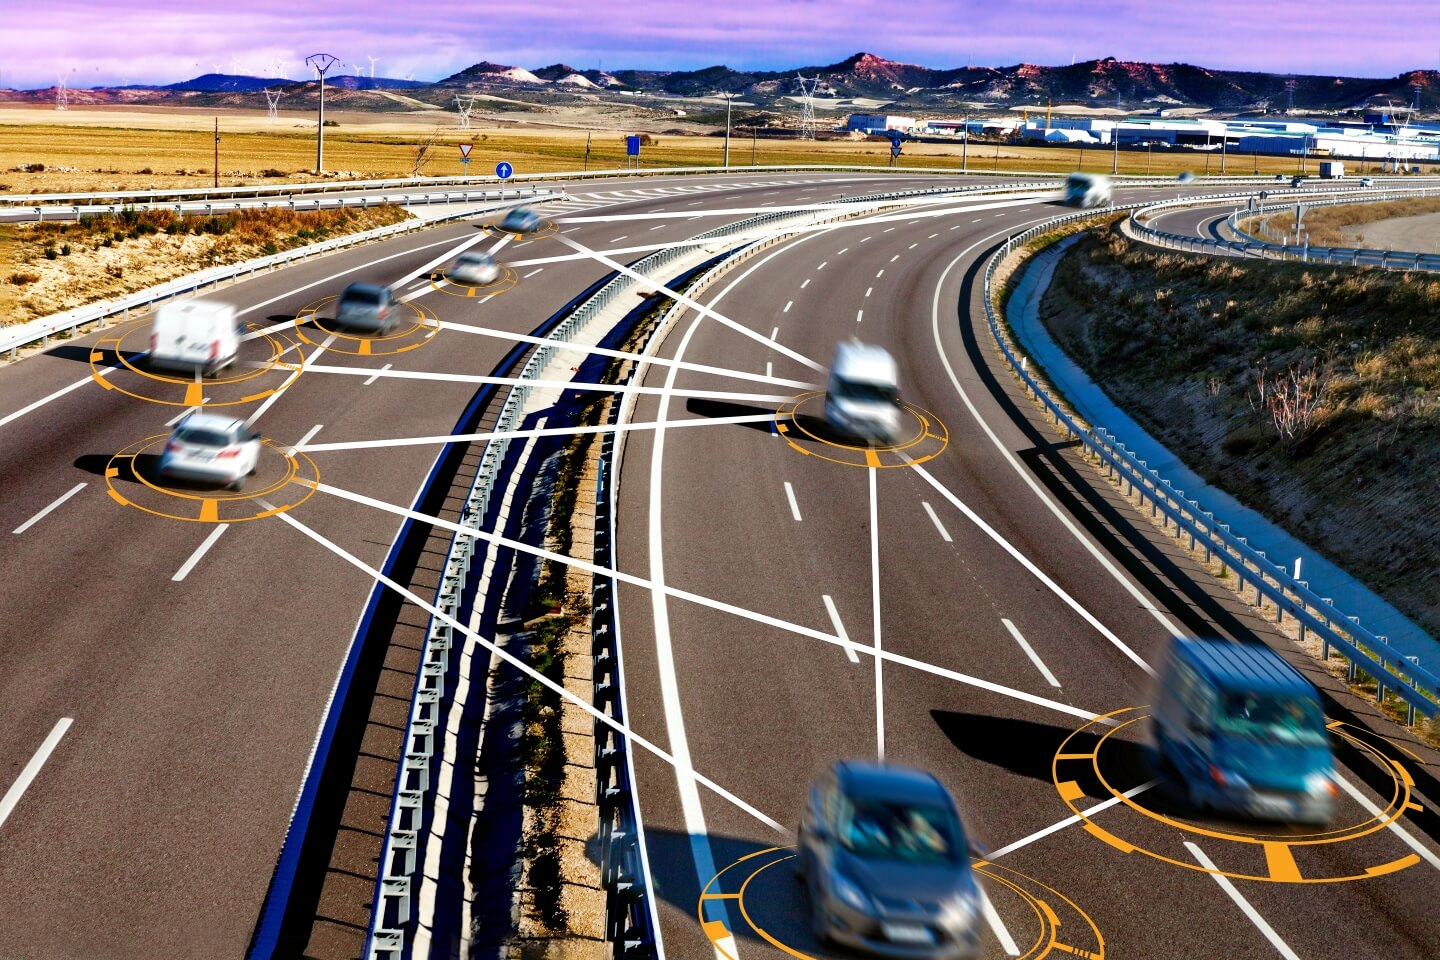
\includegraphics[width=\linewidth,height=14cm,keepaspectratio]{imagen_ejemplo.jpeg}\\[2pt]
  {\sffamily\fontsize{18}{22}\selectfont\color{muted}Figura 1. Ejemplo de contexto (reemplazar).}
\end{center}

\vfill
\seccion{Resultados y validación}

\lipsum[8][1-6]

\begin{center}
  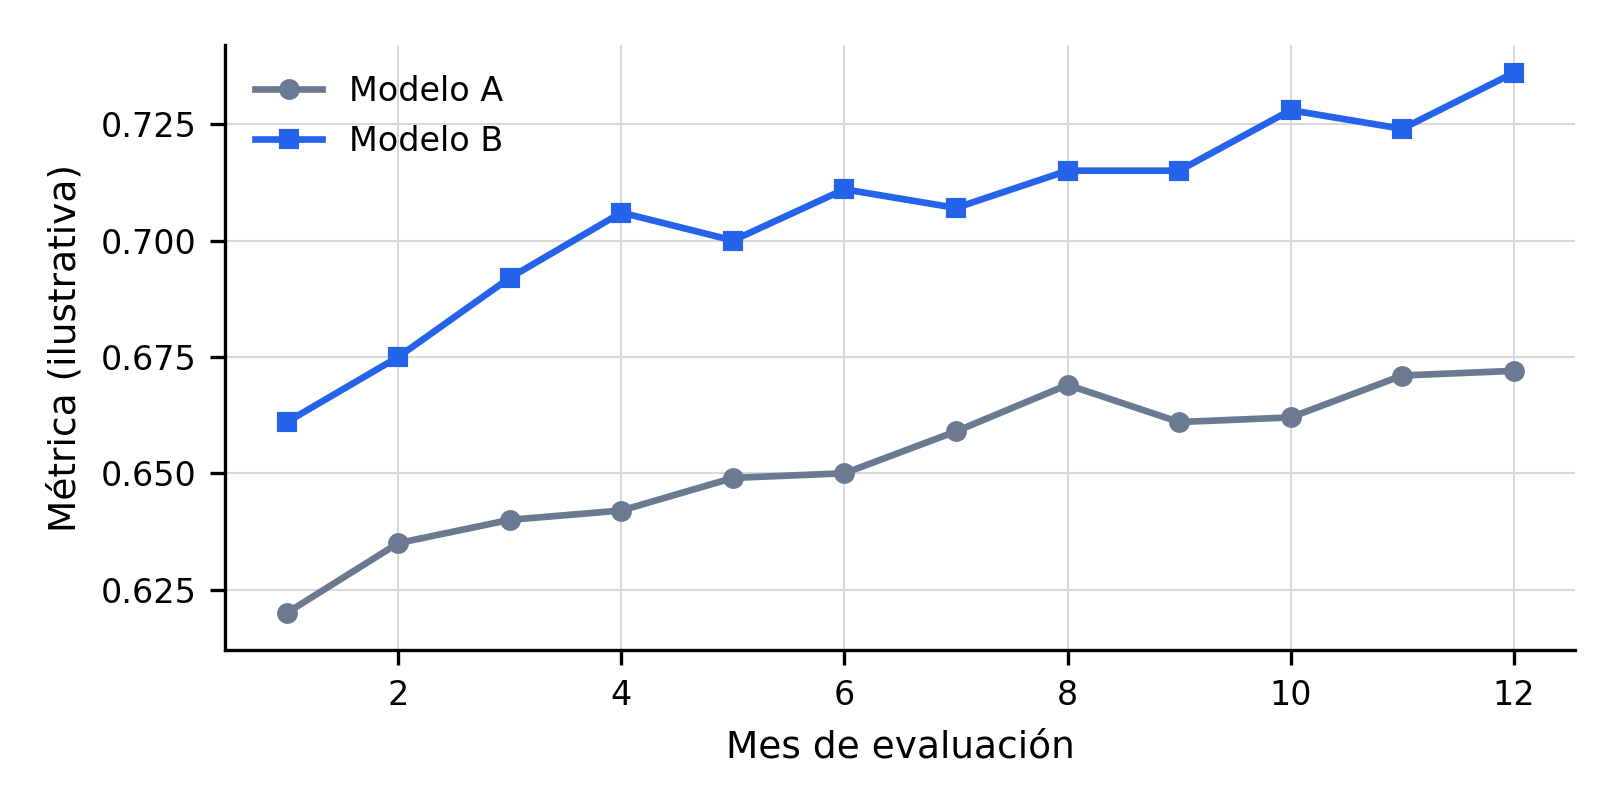
\includegraphics[width=0.95\linewidth,height=9cm,keepaspectratio]{figura_ejemplo.png}\\[2pt]
  {\sffamily\fontsize{18}{22}\selectfont\color{muted}Figura 2. Ejemplo de resultado (reemplazar).}
\end{center}

\vfill
\seccion{Arquitectura de despliegue}
\begin{center}
\begin{tikzpicture}[
  paso/.style={align=center,font=\sffamily\bfseries\fontsize{20}{24}\selectfont,text width=7cm},
  arr/.style={-{Stealth[length=6mm]},line width=4pt,color=olive}]
  \node[paso] (a) at (0,0)
    {\includegraphics[width=4.6cm,height=4.6cm]{example-image-b}\\[2pt]Recolección\\de datos};
  \node[paso] (b) at (8.8,0)
    {\includegraphics[width=4.6cm,height=4.6cm]{example-image-c}\\[2pt]Preprocesamiento};
  \node[paso] (c) at (17.6,0)
    {\includegraphics[width=4.6cm,height=4.6cm]{example-image-a}\\[2pt]Modelado\\con IA};
  \draw[arr] (a.east) -- (b.west);
  \draw[arr] (b.east) -- (c.west);
\end{tikzpicture}
\end{center}

\end{minipage}\hfill
\begin{minipage}[t][\colh][s]{0.30\linewidth}\cuerpo\vspace{0pt}
% ===== COLUMNA DERECHA =====

\seccion{Conclusiones clave}
\lipsum[10][1-6]

\begin{center}
{\sffamily\fontsize{18}{22}\selectfont\color{muted}Tabla 1. Comparación de modelos.}

\vspace{0.3em}
\fontsize{22}{28}\selectfont
\renewcommand{\arraystretch}{1.4}
\arrayrulecolor{olivedark}
\begin{tabular}{lcc}
  \toprule
  \textbf{Modelo} & \textbf{Precisión} & \textbf{F1} \\
  \midrule
  Modelo A & 0.91 & 0.89 \\
  Modelo B & 0.87 & 0.85 \\
  Modelo C & 0.93 & 0.92 \\
  \bottomrule
\end{tabular}
\end{center}

\lipsum[9][1-8]


\vfill
\seccion{Trabajo futuro}
\lipsum[11][1-5]

\vspace{0.4em}
\begin{center}
  \circulo{Análisis\\sistemático}\hspace{0.2cm}
  \circulo{Identificación\\de hallazgos}\hspace{0.2cm}
  \circulo{Propuesta\\de solución}
\end{center}

\vfill
\seccion{Referencias}
{\fontsize{18}{23}\selectfont
\begin{itemize}[leftmargin=1.2em,itemsep=0.3em]
  \item Apellido, A., y Apellido, B. (2021). \emph{Título del artículo de ejemplo.} Revista de Ejemplo, 12(3), 100--120.
  \item Apellido, C., Apellido, D., y Apellido, E. (2022). \emph{Otro título de ejemplo sobre el tema.} Journal of Example, 45, 55--70.
  \item Apellido, F. (2023). \emph{Tercer artículo de referencia.} Conferencia de Ejemplo, 200--210.
  \item Apellido, G., y Apellido, H. (2020). \emph{Cuarto título de ejemplo.} Revista de Ejemplo, 8(1), 15--32.
  \item Apellido, I. (2022). \emph{Quinto título de referencia.} Editorial de Ejemplo.
\end{itemize}}

\end{minipage}

\vfill
% ---------------------- DECLARACIÓN DE IA ------------------
{\color{olive}\rule{\linewidth}{2.5pt}}
\vspace{0.3cm}

\noindent
{\fontsize{18}{23}\selectfont\color{ink}
{\serif\color{olivedark}\fontsize{22}{28}\selectfont Declaración de uso de inteligencia artificial.}
Se utilizó \textcolor{red}{Herramienta para [indicar la finalidad]}.
La responsabilidad final sobre el contenido entregado recae en los autores.\par}

\end{document}
